\chapter{软件设计与实现}

本章将阐述农业果实称重云端软件的软件架构设计、数据库设计、称重数据处理流程设计以及农场数据管理功能设计。

\section{软件架构设计}\label{sec:architecture}

农业果实称重云端软件的整体架构采用边端+远端协同的模式进行设计,将靠近农场端的服务称为边端服务,远离农场端的服务称为远端服务,其中边端服务一般部署在农场局域网内,在网络受限的情况下,确保称重流程的正常进行。整体软件部署架构图如图\ref{fig:软件部署架构图}所示。

\begin{figure}[H]
    \centering
    \includegraphics[width=0.8\linewidth]{../design/out/软件部署架构图.png}
    \caption{软件部署架构图}
    \label{fig:软件部署架构图}
\end{figure}

如图\ref{fig:软件部署架构图}所示,存在三个端,分别是边端、远端以及前台网页端,它们分别部署在三台不同服务器上。其中边端可以代表某一个农场,可以有多个农场边端同时连接到远端服务器。下面根据该部署架构,描述电子秤提交称重数据的通信流程:

1、首先由电子秤拍摄果实图片,然后果实识别模块对果实种类进行识别并将果实图片存储至边端 MinIO 对象存储库,最后电子秤通过自身所支持的通信协议向网关提交称重数据;

2、网关处理电子秤的发出的请求,通过 EMQX 协议转换技术完成协议转换,通过读取 MySQL 从库数据完成电子秤信息认证和授权,最后将数据以 MQTT 协议的格式发送至 MQTT Broker 集群;

3、MQTT Broker 接收到 MQTT 消息后,该集群内任一节点都可以处理请求并将消息持久化;

4、远端服务订阅 MQTT Broker 集群中所有节点的消息,收到消息后进行消息解析,通过边端 MinIO 对象存储读取果实图片并持久化至本地 MinIO 对象存储。如果果实种类未知,则通过果实识别服务根据果实图像识别出果实种类。最后将称重处理的结果写入 MySQL 主库。

5、至此已经完成称重数据的处理。此外,在后台管理界面,员工可以查看历史称重记录,管理员可以在待办界面处理待办,手动填写并提交处理失败的称重数据。

该架构主要的优势是实现了两端数据处理的独立性,对于边端,不管是提交称重数据还是存储果实图片,都只需在边端完成,不仅提高了数据处理速度,而且在网络受限的情况下也不会影响称重数据的处理。对于远端,则只需要订阅称重消息进行处理即可。下面进一步分析软件架构的特点,可以得到软件的分层架构图,如图\ref{fig:软件分层架构图}所示。

\begin{figure}[H]
    \centering
    \includegraphics[width=0.8\linewidth]{../design/out/软件分层架构图.png}
    \caption{软件分层架构图}
    \label{fig:软件分层架构图}
\end{figure}

软件可以抽象出五个层级,分别是表现层、通信层、网关层、服务层、数据层。各层作用如下:

1、表现层:该层可以理解为接口调用者,包含前台网页端和电子秤,两者都通过调用后台提供的接口来完成数据的处理或展示;

2、通信层:该层服务于表现层和网关层之间的通信。软件所支持的通信协议有四种,分别是 HTTP/HTTPS、MQTT、CoAP 和 STOMP。其中前台网页端可以通过 HTTP/HTTPS 调用后台接口,而电子秤可以通过四种协议中任一一种来提交称重数据;

3、网关层:该层提供了接口路由和协议转换功能。表现层发来的请求根据接口路由导向服务层中对应的服务,协议转换功能则服务于电子秤,将不同协议统一转为 MQTT 协议,以 MQTT 协议继续进行后续通信;

4、服务层:该层完成具体的数据服务逻辑。包含四大模块,用户模块、果实模块、作业模块以及称重模块,各个模块相互依赖,共同协作,完成数据的查询和处理;

5、数据层:该层完成数据的持久化和缓存操作。MySQL 数据库用于持久化数据;Redis 数据库用于实现数据缓存功能;MQTT Broker 类似于消息队列,用于临时存储 MQTT 消息;MinIO 是对象存储库,主要用于储存果实图片,其中边端对象存储库用于临时存储果实图片,如果 MQTT Broker 中的称重消息和后台管理中的待办记录均以被清空,则可进行数据处理以节省存储成本,相对的,远端对象存储库则持久化地存储果实图片,用于后续进一步的分析;

综上所述,根据软件部署架构图\ref{fig:软件部署架构图}可以得到软件整体的通信流程和部署思路,根据软件分层架构图\ref{fig:软件分层架构图}可以清晰地划分出功能模块,更高效地进行后续软件的开发。

\section{数据库设计}\label{sec:database}

软件数据库设计分为三个阶段:概念模型设计、逻辑模型设计和物理模型设计,在\ref{sec:req1}中,通过对需求的分析完成了数据建模,给出了软件中存在的实体及实体关系,也即完成了数据库中概念模型的设计。下面进行数据库的逻辑模型设计和物理模型设计。

基于图\ref{fig:ERD}所展示的实体关系以及功能权限表\ref{tab:user_permissions}所展示的用户功能权限信息,下面阐述逻辑模型设计,描述系统各个表的结构及其字段定义,涵盖了表之间的关系、字段的数据类型及约束条件,如表\ref{tab:user},表\ref{tab:produce},表\ref{tab:work},表\ref{tab:scale},表\ref{tab:record},表\ref{tab:todo},表\ref{tab:mqttacl}所示。

% t_user
\begin{longtblr}
    [
    caption        = {用户表 (t\_user)},
    label          = {tab:user}
    ]
    {
        colspec={Q[c,m]X[c,m]},
        hlines,vlines,cell{2-Z}{1}={},
        row{1}         = {font=\bfseries},
        rowhead        = 1,
    }
    字段 & 类型 & 约束 & 说明 \\
    id & bigint & 主键 & 自增主键 \\
    uid & varchar(255) & 非空,唯一 & 用户认证编号 \\
    name & varchar(255) & 非空 & 用户名称 \\
    password & varchar(255) & 非空 & 密码(加密) \\
    roles & varchar(255) & - & 角色(英文逗号分隔) \\
    create\_time & bigint & 非空 & 创建时间(毫秒级时间戳) \\
    update\_time & bigint & 非空 & 更新时间(毫秒级时间戳) \\
    status & int & 非空 & 状态(0禁用/1启用/2已删除) \\
\end{longtblr}

表\ref{tab:user}中展现了软件中用户实体的具体字段设计,其中 roles 字段定义了用户角色,角色字段包含管理员(ROLE\_ADMIN)、采摘员工(ROLE\_EMPLOYEE)、电子秤(ROLE\_SCALE)以及系统用户(ROLE\_SYS),如果用户包含多个角色,则使用英文半角逗号隔开。

% t_produce
\begin{longtblr}
    [
    caption        = {果实表 (t\_produce)},
    label          = {tab:produce}
    ]
    {
        colspec={Q[c,m]X[c,m]},
        hlines,vlines,cell{2-Z}{1}={},
        row{1}         = {font=\bfseries},
        rowhead        = 1,
    }
字段 & 类型 & 约束 & 说明 \\
id & bigint & 主键 & 系统自带从0开始,用户添加从1000000开始 \\
name & varchar(255) & 非空,唯一 & 果实名称 \\
name\_en & varchar(255) & 唯一 & 果实英文名称 \\
create\_time & bigint & 非空 & 创建时间(毫秒级时间戳) \\
update\_time & bigint & 非空 & 更新时间(毫秒级时间戳) \\
status & int & 非空 & 状态(0未种植/1在种植/2已删除) \\
\end{longtblr}

表\ref{tab:produce}中展现了软件中果实实体的具体字段设计。

% t_work
\begin{longtblr}
    [
    caption        = {采摘作业表 (t\_work)},
    label          = {tab:work}
    ]
    {
        colspec={Q[c,m]X[c,m]},
        hlines,vlines,cell{2-Z}{1}={},
        row{1}         = {font=\bfseries},
        rowhead        = 1,
    }
字段 & 类型 & 约束 & 说明 \\
id & bigint & 主键 & 自增主键 \\
produce\_id & bigint & 非空 & 果实编号 \\
start\_time & bigint & 非空 & 采摘开始时间(毫秒级时间戳) \\
end\_time & bigint & 非空 & 采摘结束时间(毫秒级时间戳) \\
data\_value & decimal(10,2) & - & 总的采摘称重结果 \\
unit & int & - & 称重单位(0mg/1g/2kg/3t/4lb/5oz/6ct) \\
create\_time & bigint & 非空 & 创建时间(毫秒级时间戳) \\
update\_time & bigint & 非空 & 更新时间(毫秒级时间戳) \\
status & int & 非空 & 状态(0未开始/1进行中/2已结束/3已取消/4已删除) \\
\end{longtblr}

表\ref{tab:work}中展现了软件中采摘作业实体的具体字段设计。其中通过字段果实编号(produce\_id)关联了果实实体,字段对应果实表\ref{tab:produce}中的 id 字段。

% t_scale
\begin{longtblr}
    [
    caption        = {电子秤表 (t\_scale)},
    label          = {tab:scale}
    ]
    {
        colspec={Q[c,m]X[c,m]},
        hlines,vlines,cell{2-Z}{1}={},
        row{1}         = {font=\bfseries},
        rowhead        = 1,
    }
字段 & 类型 & 约束 & 说明 \\
id & bigint & 主键 & 自增主键 \\
sid & varchar(255) & 非空 & MQTT 用户认证编号 \\
model & varchar(255) & - & 型号 \\
max\_capacity & decimal(10,2) & 非空 & 最大量程 \\
min\_capacity & decimal(10,2) & 非空 & 最小量程 \\
unit & int & 非空 & 量程单位(0mg/1g/2kg/3t/4lb/5oz/6ct) \\
verification\_interval & int & - & 检定分度值 \\
display\_interval & int & - & 显示分度值 \\
unit\_dv & int & - & 分度值单位(0mg/1g/2kg/3t/4lb/5oz/6ct) \\
protocol & varchar(255) & - & 协议(小写,逗号分隔) \\
create\_time & bigint & 非空 & 创建时间(毫秒级时间戳) \\
update\_time & bigint & 非空 & 更新时间(毫秒级时间戳) \\
status & int & 非空 & 状态(0禁用/1启用/2已删除) \\
\end{longtblr}

表\ref{tab:scale}中展现了软件中电子秤实体的具体字段设计。其中通过字段电子秤编号(sid)管理了用户实体,该字段对应于用户表\ref{tab:user}中的用户编号(uid)字段。

% t_record
\begin{longtblr}
    [
    caption        = {称重记录表 (t\_record)},
    label          = {tab:record}
    ]
    {
        colspec={Q[c,m]X[c,m]},
        hlines,vlines,cell{2-Z}{1}={},
        row{1}         = {font=\bfseries},
        rowhead        = 1,
    }
字段 & 类型 & 约束 & 说明 \\
id & bigint & 主键 & 自增主键 \\
work\_id & bigint & 非空 & 采摘作业编号 \\
produce\_id & bigint & 非空 & 果实编号 \\
image & varchar(255) & - & 果实图片地址 \\
employee\_id & bigint & 非空 & 员工编号 \\
scale\_id & bigint & 非空 & 电子秤编号 \\
data\_value & decimal(10,2) & 非空 & 称重结果 \\
data\_error\_margin & decimal(10,2) & - & 称量结果误差范围 \\
unit & int & 非空 & 称重单位(0mg/1g/2kg/3t/4lb/5oz/6ct) \\
data\_time & bigint & 非空 & 称重时间(毫秒级时间戳) \\
\end{longtblr}

表\ref{tab:record}中展现了软件中称重记录实体的具体字段设计。通过字段果实编号(produce\_id)关联了果实实体,对应果实表\ref{tab:produce}中的 id 字段;通过字段采摘作业编号(work\_id)关联了作业实体,对应作业表\ref{tab:work}中的 id 字段;通过字段员工编号(employee\_id)关联了员工实体,对应用户表\ref{tab:user}中的 id 字段;通过字段电子秤编号(scale\_id)关联了电子秤实体,对应电子秤表\ref{tab:scale}中的 id 字段。

% t_todo
\begin{longtblr}
    [
    caption        = {待处理称重记录表 (t\_todo)},
    label          = {tab:todo}
    ]
    {
        colspec={Q[c,m]X[c,m]},
        hlines,vlines,cell{2-Z}{1}={},
        row{1}         = {font=\bfseries},
        rowhead        = 1,
    }
字段 & 类型 & 约束 & 说明 \\
id & bigint & 主键 & 自增主键 \\
produce\_id & bigint & - & 果实编号 \\
produce\_name & varchar(255) & - & 果实名称 \\
image & varchar(255) & - & 采摘作业图片地址 \\
employee\_id & bigint & 非空 & 员工编号 \\
scale\_id & bigint & 非空 & 电子秤编号 \\
data\_value & decimal(10,2) & 非空 & 称重结果 \\
data\_error\_margin & decimal(10,2) & - & 称量结果误差范围 \\
unit & int & 非空 & 称重单位(0mg/1g/2kg/3t/4lb/5oz/6ct) \\
data\_time & bigint & 非空 & 称重时间(毫秒级时间戳) \\
\end{longtblr}

表\ref{tab:todo}中展现了软件中待办记录实体的具体字段设计。通过字段果实编号(produce\_id)关联了果实实体,对应果实表\ref{tab:produce}中的 id 字段;通过字段员工编号(employee\_id)关联了员工实体,对应用户表\ref{tab:user}中的 id 字段;通过字段电子秤编号(scale\_id)关联了电子秤实体,对应电子秤表\ref{tab:scale}中的 id 字段。

% t_mqtt_acl
\begin{longtblr}
    [
    caption        = {MQTT 访问控制表 (t\_mqtt\_acl)},
    label          = {tab:mqttacl}
    ]
    {
        colspec={Q[c,m]X[c,m]},
        hlines,vlines,cell{2-Z}{1}={},
        row{1}         = {font=\bfseries},
        rowhead        = 1,
    }
字段 & 类型 & 约束 & 说明 \\
id & int & 主键 & 自增主键 \\
username & varchar(255) & 非空 & MQTT 认证用户名 \\
permission & varchar(255) & 非空 & 操作权限(allow/deny,即允许/拒绝) \\
action & varchar(255) & 非空 & 操作类型(publish/subscribe/all,即发布/订阅/所有) \\
topic & varchar(255) & 非空 & 适用主题 \\
qos & int & - & 消息 QoS 级别(0,1,2) \\
retain & int & - & 是否支持发布保留消息(0否/1是) \\
\end{longtblr}

表\ref{tab:mqttacl}中展现了软件中 MQTT 服务的访问控制条目的具体字段设计。通过字段 MQTT 认证用户名(username)管理了用户实体,对应用户表\ref{tab:user}中的 uid 字段。

数据库中每个表的设计都遵循规范化原则,以确保数据的一致性、完整性和高效性。字段的定义包括主键、唯一约束、非空约束等,考虑到更新数据的效率问题,取消了外键的设置,在后台服务中做相关数据更新的限制以确保数据一致性。

基于上述数据库的逻辑模型设计,下面继续完成物理模型的设计。

软件使用 MySQL 作为数据库管理系统,采用 InnoDB 存储引擎,将事务隔离级别设置为可重复读,以确保数据的一致性和可靠性。下面从索引设计、数据存储与分布、数据访问控制和事务日志与恢复策略四个方面阐述物理模型设计。

索引设计方面:针对实际业务场景,基于逻辑模型设计中的表信息,设置了相关索引以提高查询更新效率,如表\ref{tab:index}所示。

% INDEX
\begin{longtblr}
    [
    caption        = {索引设计表 (INDEX)},
    label          = {tab:index}
    ]
    {
        colspec={Q[c,m]X[c,m]},
        hlines,vlines,cell{2-Z}{1}={},
        row{1}         = {font=\bfseries},
        rowhead        = 1,
    }
表 & 索引字段 & 说明 \\

t\_record & scale\_id & 高效查找电子秤历史称重记录 \\

t\_record & employee\_id & 高效查找员工历史称重记录 \\

t\_record & employee\_id, work\_id & 高效查找员工各采摘作业批次历史称重记录 \\

t\_record & work\_id & 高效查找各采摘作业批次历史称重记录 \\

t\_work & produce\_id & 高效查找果实对应的采摘作业 \\
\end{longtblr}

数据存储与分布方面:采用主从架构,在靠近农场边端部署从库,在远端服务器部署主库,主从库采用\ref{sec:gtid}中提到的基于 GTID 的主从复制技术完成数据实时同步。

数据访问控制方面:主库允许读写,而从库只允许读,屏蔽任何用户的写操作,确保数据一致性。

事务日志与恢复策略方面:主从库均开启 BinLog(二进制日志)。在上述数据复制技术中,从库通过读取主库的二进制日志来同步数据。除此之外,在数据丢失或损坏的情况下,通过回放二进制日志来恢复丢失的数据。

\section{称重数据处理流程设计与实现}\label{sec:weigh-process}

软件采用远边协同的方式来处理称重数据,称重数据先在边端(即离电子秤较近的一端)完成提交,然后远端通过订阅的模式完成后续的数据处理和持久化,下面将介绍具体的数据处理流程。首先对边端数据处理的流程进行阐述,如图\ref{fig:边端称重数据处理流程活动图}所示。

\begin{figure}[H]
    \centering
    \includegraphics[width=0.8\linewidth]{../design/out/边端称重数据处理流程活动图.png}
    \caption{边端称重数据处理流程活动图}
    \label{fig:边端称重数据处理流程活动图}
\end{figure}

图\ref{fig:边端称重数据处理流程活动图}展现了以采摘员工、电子秤和边端服务为参与对象的活动泳道,描述了称重数据在边端向 MQTT Broker 的提交流程。其具体流程是:

1、采摘员工放置果实在电子秤上,然后刷员工卡;

2、电子秤对果实完成称重操作获取到称重结果,同时完成员工卡数据的读取,读取失败则返回错误信息,员工需要确认电子秤状态或者员工卡信息是否异常,然后选择重试或取消称重;

3、电子秤成功读取卡和称重数据后,拍摄并识别果实,然后储存果实图片,接着生成称重信息,开始尝试提交到边端服务的网关处;

4、边端服务的网关收到电子秤消息,首先完成协议转换,转换失败则返回错误信息,跳转到第 7 步;

5、转换成功后,进行认证授权操作。先进行认证,通过电子秤编号和密码完成认证,接着根据电子秤编号查询 MQTT 用户授权信息,确认电子秤是否有相关主题的发布功能。认证授权失败则返回错误信息,跳转到第 7 步;

6、认证授权成功后,即发布消息到 MQTT Broker,根据发布结果返回成功或失败信息;

7、如果提交成功或者重试次数超过电子秤设置的重试次数阈值,则退出第 3 步到第 7 步到循环,显示称重结果;

8、判断称重是否成功,如果成功则完成果实入库,否则返回第 1 步。

称重数据在边端完成提交并且称重消息在 MQTT Broker 处完成持久化后,便视为称重完成。接下来由监控 Broker 的远端服务对称重数据进一步处理,如远端称重数据处理流程活动图\ref{fig:远端称重数据处理流程活动图}所示。

\begin{figure}[H]
    \centering
    \includegraphics[width=0.8\linewidth]{../design/out/远端称重数据处理流程活动图.png}
    \caption{远端称重数据处理流程活动图}
    \label{fig:远端称重数据处理流程活动图}
\end{figure}

如图\ref{fig:远端称重数据处理流程活动图}所示,显示了远端接收相关称重消息后,称重消息在后台服务中的处理控制流程。具体步骤是:

1、远端服务的 MQTT 客户端接收到消息后,首先检查数据中员工和电子秤状态是否处于启用状态,如果不是则进入第 6 步;

2、根据图片识别果实,如果识别失败则进入第 6 步;

3、查询果实对应的采摘作业,如果不存在,则进入第 6 步;

4、检查作业和果实状态是否处于启用状态,如果不是则进入第 6 步;

5、前面步骤中没有发生异常,则持久化称重信息并发布处理成功的消息到 MQTT Broker,数据处理完成;

6、处理过程中发生异常,为防止数据丢失,将称重消息写入待办并发布处理失败的消息到 MQTT Broker。在管理后台待办界面中,由管理员人工完成异常称重数据的处理。

在上述称重数据的处理流程中,存在两个需要注意的问题:

(1)关于称重数据处理结果的订阅:在最后称重数据处理成功或失败结果的消息发布到 MQTT Broker 之后,可以由特定的监控者订阅相关主题,进行告警或其它相关操作。在本软件中,通过电子秤模拟器对该结果进行订阅,而实际生产中需要注意电子秤不需要关心这个数据处理的结果,只要电子秤在边端完成称重数据的提交,电子秤就将称重操作视做成功;

(2)关于 MQTT 消息的配置问题:边端和远端称重消息在 MQTT Broker 进行发布和订阅时,需要考虑 MQTT 消息的配置问题。对于消息主题的设置,发布/订阅称重消息和发布/订阅称重数据处理结果消息应该属于两个不同主题;对于传输质量级别的设置,需要确保消息有且仅被消费一次。根据\ref{sec:mqtt}中提到的三种 QoS 级别,这里应该选择 QoS2 级别,确保称重数据的可靠传输;

结合上述对远端和边端称重数据处理流程的设计和分析,可以作为代码编写的主要基础。

\begin{figure}[H]
    \centering
    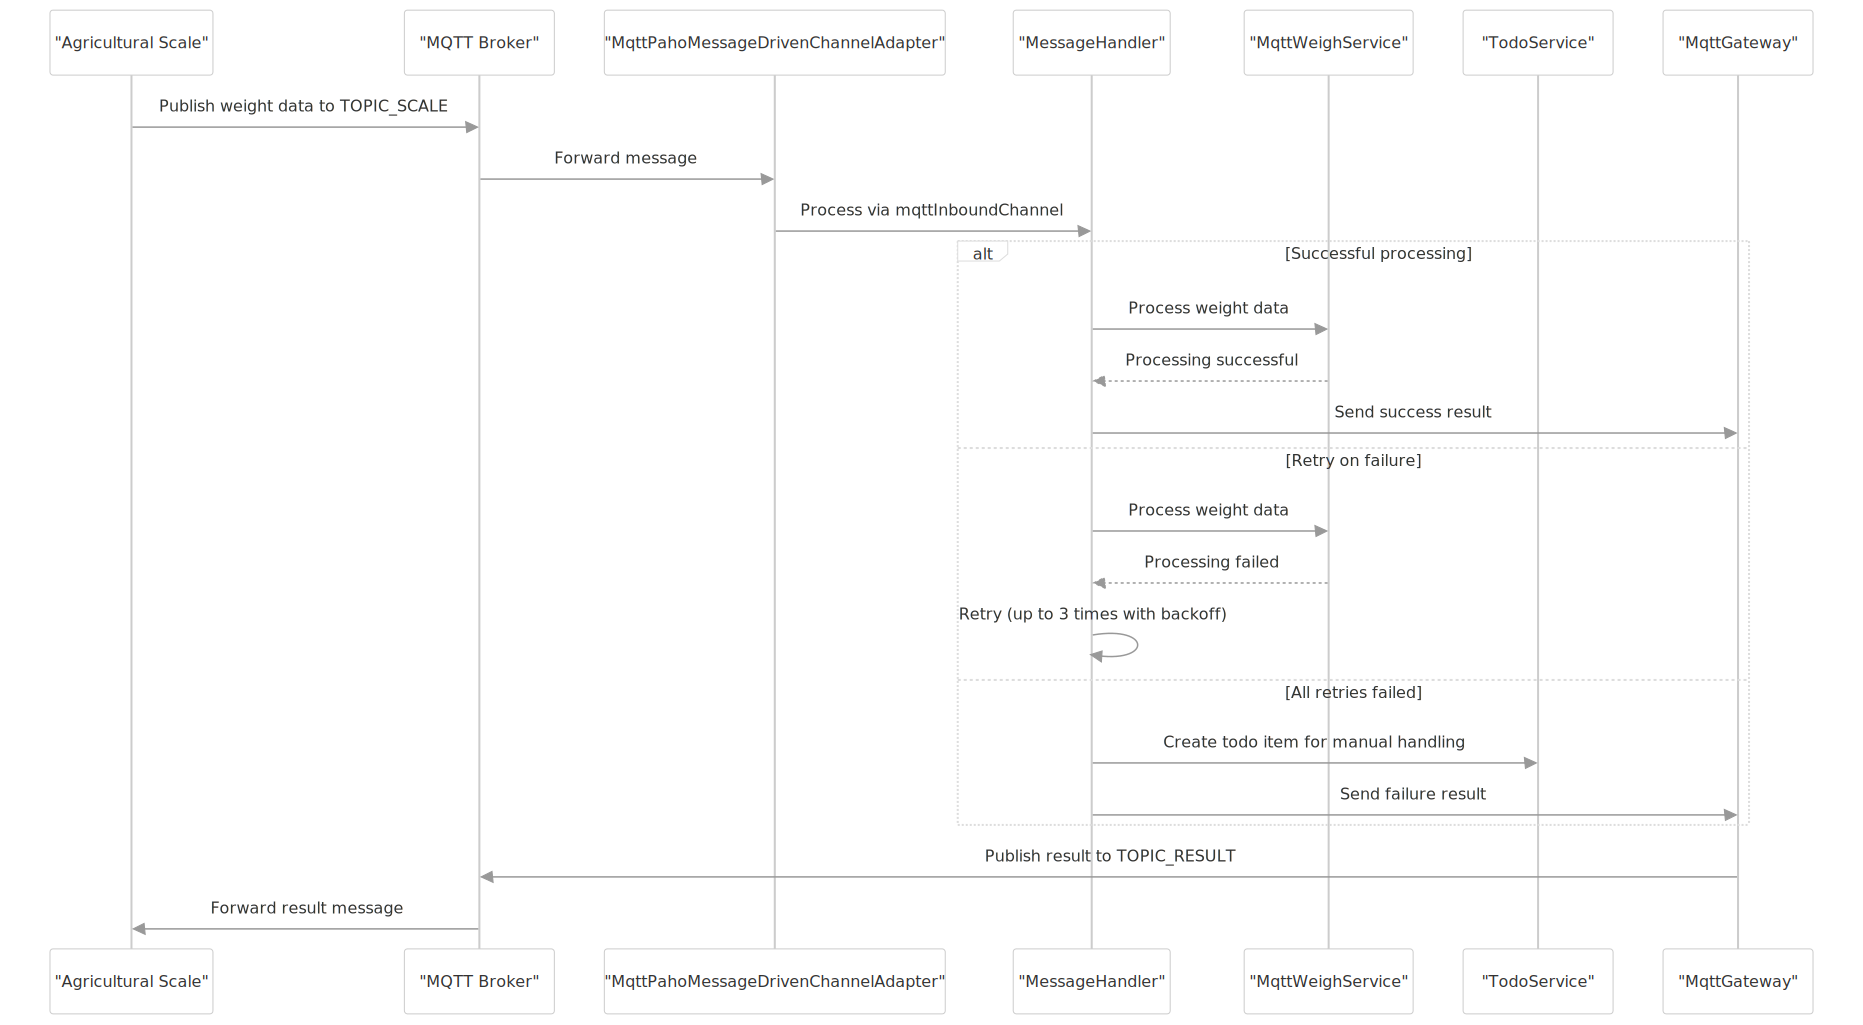
\includegraphics[width=0.9\linewidth]{../design/test.png}
    \caption{test}
    \label{fig:test}
\end{figure}

\section{农场数据管理功能设计与实现}\label{data-management}

农业果实称重云端软件主要管理五种数据,分别是电子秤、果实、采摘作业、用户、待办数据和称重数据。下面分别对这些数据的管理功能进行阐述。

对于电子秤,软件对其提供基本的增删改查操作,除此之外还提供对每个电子秤历史称重数据的查询和导出。对于电子秤接入云端软件的注册流程,这里进行具体的阐述。电子秤的注册流程如下:

(1) 管理员登入后台管理系统-电子秤管理模块;

(2) 填写电子秤信息,包含电子秤密钥、规格等信息,填写完成后提交;

(3) 写入电子秤表并注册 MQTT 用户,为电子秤添加发布称重消息到称重主题(t/scale)的权限;

(4) 至此电子秤接入完成,可以开始进行称重数据的提交。

对于果实,软件对其提供基本的增删改查操作,除此之外还提供对每种果实年产量数据、分批次采摘量数据的可视化和导出功能。软件内置了超二十种果实种类,通过读取果实图像识别模型的训练配置文件,在数据库果实表初始化了支持识别的果实,管理员可以根据农场实际情况,修改果实状态为种植中或未种植。如果需要添加新的果实,具体操作流程如下:

(1) 准备新果实数据集,基于原模型继续训练模型;

(2) 模型训练完成后,重启果实识别服务;

(3) 读取训练配置文件,自动完成新种类果实的写入;

(4) 管理员在管理后台根据农场实际情况,更新果实种植状态。

对于采摘作业,软件对其提供基本的增删改查操作,除此之外还提供导出所有采摘作业数据的功能。采摘作业的状态包含未开始、进行中、已结束、已取消和已删除,采用 Spring 定时任务的功能,每 5s 检查在未开始和进行中状态作业,根据当前时间更新作业状态为进行中或已结束状态。此外,对采摘作业的提交,其处理流程如图\ref{fig:新建采摘作业流程图}所示。

\begin{figure}[H]
    \centering
    \includegraphics[width=0.8\linewidth]{../design/out/新建采摘作业流程图.png}
    \caption{新建采摘作业流程图}
    \label{fig:新建采摘作业流程图}
\end{figure}

如图\ref{fig:新建采摘作业流程图}所示,新建采摘作业具体流程是:

(1) 管理员点击新建采摘作业,完成编辑和提交;

(2) 后台首先检查时间是否合法,如果不合法则抛出异常,结束流程;

(3) 检查要采摘的果实是否处在种植状态,如果不是则抛出异常,结束流程;

(4) 检查要采摘的果实是否已经存在进行中的采摘作业,如果有则抛出异常,结束流程;

(5) 采摘作业校验通过,根据采摘时间和当前时间,设置采摘状态为进行中或未开始;

(6) 将采摘作业写入数据库,结束流程。

对于用户,软件对其提供基本的增删改查操作,除此之外提供对于采摘员工的分批采摘量数据和称重历史数据的统计和导出功能。软件中包含了四类用户,分别是采摘员工、管理员、电子秤和系统用户,其中电子秤用户不可登入后台管理界面,系统用户则作为一种特殊的用户,用于订阅称重主题相关的消息并进行处理,为软件自带的用户。

对于待办数据,软件对其提供基本的增删查操作。管理员可以在后台管理中的待办管理模块,完成待办的提交或丢弃。此外,为提高数据处理的效率,提供了批量提交和丢弃功能。对于批量提交功能,管理员可以在待办列表中同时选中多个相同种类果实的称重数据,然后点击批量提交,一次完成多条数据的处理。对于待办记录的处理,遵循如图\ref{fig:待办记录处理流程图}的流程:

\begin{figure}[H]
    \centering
    \includegraphics[width=0.8\linewidth]{../design/out/待办记录处理流程图.png}
    \caption{待办记录处理流程图}
    \label{fig:待办记录处理流程图}
\end{figure}

如图\ref{fig:待办记录处理流程图},具体的操作流程是:

(1) 管理员编辑待办并点击提交;

(2) 检查记录是否存在果实名称或编号,如果存在则进入第 5 步;

(3) 检查记录是否存在果实图片,如果不存在则进入第 8 步;

(4) 根据果实图片识别果实种类,如果识别失败则进入第 8 步;

(5) 查询果实对应采摘作业,如果没找到则进入第 8 步;

(6) 检查果实和作业状态,如果果实不处在种植状态或者作业不处在进行中状态,则进入第 8 步;

(7) 持久化称重记录,处理成功,结束流程;

(8) 处理失败,抛出异常,结束流程。

对于称重数据,软件对其提供基本的增查操作。在\ref{sec:weigh-process}中对称重数据的处理进行了具体的阐述,而在数据管理方面,称重数据会持久性的进行存储,方面进一步的数据统计与分析。对于称重数据的存储管理问题,由于称重数据中的果实图片往往占用较多空间,因此需要尤其注意图片数据的存储。在称重流程中,果实图片首先临时存储在边端对象存储库,远端读取称重消息时,将果实图片下载至本地进行持久化。其中由于边端可能存在存储受限的问题,所以每隔一段时间进行图片数据的清理,具体的清除触发条件是:

(1) 存储空间超过 80\%;

(2) MQTT Broker 中的称重消息没有积压,已经全部完成读取;

(3) 软件中不存在未处理的待办记录。

边端自动化程序将每隔 1h 检查上述三个条件,如果均满足,则进行对象存储库的清理操作。清理过程中禁止新的对象写入,防止出现数据不一致的问题。

% \section{服务接口设计}

% \begin{table}[H]
% \centering
% \caption{称重模块接口设计}
% \label{tab:interface-weigh}
% \begin{tabular}{|c|c|c|}
% \hline
% 接口名称 & 请求方法 & 接口路径 \\\hline
% 更新电子秤信息 & PUT & /weigh/scale \\ \hline
% 添加电子秤 & POST & /weigh/scale \\\hline
% 添加称重记录 & POST & /weigh/record \\\hline
% 提交待处理称重记录 & POST & /weigh/record/todo \\\hline
% 丢弃待处理称重记录 & DELETE & /weigh/record/todo \\\hline
% 获取待处理称重记录 & GET & /weigh/record/todo/list \\\hline
% 获取称重记录 & POST & /weigh/record/list \\\hline
% 添加称重结果监控者 & POST & /weigh/monitor \\\hline
% 获取员工各作业采摘量 & GET & /weigh/summary \\\hline
% 获取电子秤 & GET & /weigh/scale/{id} \\\hline
% 获取电子秤列表 & GET & /weigh/scale/list \\\hline
% \end{tabular}
% \end{table}
% 表\ref{tab:interface-weigh}显示了称重模块的接口设计,各接口以 /weigh 作为前缀。

% \begin{table}[H]
% \centering
% \caption{用户模块接口设计}
% \label{tab:interface-user}
% \begin{tabular}{|c|c|c|}
% \hline
% 接口名称 & 请求方法 & 接口路径 \\ \hline
% 用户获取个人信息 & GET & /user \\ \hline
% 管理员更新用户 & PUT & /user \\ \hline
% 管理员添加用户 & POST & /user \\ \hline
% 用户更新个人信息 & PUT & /user/me \\ \hline
% 用户登录 & POST & /user/login \\ \hline
% 管理员获取用户信息 & GET & /user/{uid} \\ \hline
% 管理员获取用户列表 & GET & /user/list \\ \hline
% \end{tabular}
% \end{table}
% 表\ref{tab:interface-user}显示了用户模块的接口设计,各接口以 /user 作为前缀。

% \begin{table}[H]
% \centering
% \caption{果实模块接口设计}
% \label{tab:interface-produce}
% \begin{tabular}{|c|c|c|}
% \hline
% 接口名称 & 请求方法 & 接口路径 \\ \hline
% 果实图像推理识别 & POST & /predict \\ \hline
% 根据名称获取果实 & GET & /produce \\ \hline
% 更新果实 & PUT & /produce \\ \hline
% 添加果实 & POST & /produce \\ \hline
% 获取果实 & GET & /produce/{id} \\ \hline
% 获取果实年产量 & GET & /produce/summary/year \\ \hline
% 获取果实分批产量 & GET & /produce/summary/work \\ \hline
% 获取果实列表 & GET & /produce/list \\ \hline
% \end{tabular}
% \end{table}
% 表\ref{tab:interface-produce}显示了果实模块的接口设计,除了果实图像推理识别接口,其它各接口以 /produce 作为前缀。

% \begin{table}[H]
% \centering
% \caption{作业模块接口设计}
% \label{tab:interface-work}
% \begin{tabular}{|c|c|c|}
% \hline
% 接口名称 & 请求方法 & 接口路径 \\ \hline
% 更新采摘作业 & PUT & /work \\ \hline
% 添加采摘作业 & POST & /work \\ \hline
% 获取采摘作业 & GET & /work/{id} \\ \hline
% 获取果实的采摘作业列表 & GET & /work/produce/{id}\\ \hline
% 获取采摘作业列表 & GET & /work/list \\ \hline
% \end{tabular}
% \end{table}
% 表\ref{tab:interface-work}显示了作业模块的接口设计,各接口以 /work 作为前缀。

\section{本章小结}

本章阐述了农业果实称重云端软件的架构设计、数据库设计、数据处理流程以及农场数据管理功能。通过软件架构设计,确保了系统的高效性和扩展性;数据库设计优化了数据存储和检索性能;数据处理流程设计保证了称重数据的准确性和实时性;农场数据管理功能则提高了农场运营的智能化和数据化管理水平。总体而言,本章为实现农业智能称重与数据管理提供了系统的技术框架。
